% Fri Aug 04 10:30:46 EDT 2023
%+++++++++++++++++++++++++++++++++++++++++++++++++++++++++++++++
% SUMMARY  :  Project Template
%          :  James Quinlan 
%          :  University of Southern Maine
%+++++++++++++++++++++++++++++++++++++++++++++++++++++++++++++++
\documentclass[12pt]{amsart} % Adjusted to 12pt for readability
% This has a default type size 10pt.  Other options are 11pt and 12pt

\usepackage{amssymb}   % Enables mathematical symbols
\usepackage{lipsum}    % Generates placeholder text
\usepackage{listings}
\usepackage{xcolor}
\usepackage{graphicx}
\usepackage{subfig}
\usepackage{lipsum}
\newtheorem{thm}{Theorem}[section]
\newtheorem{prop}[thm]{Proposition}
\newtheorem{lem}[thm]{Lemma}
\newtheorem{cor}[thm]{Corollary}

% Math notation
\newcommand{\R}{\ensuremath{\mathbb R}}
\newcommand{\Q}{\ensuremath{\mathbb Q}}
\newcommand{\Z}{\ensuremath{\mathbb Z}}
\newcommand{\N}{\ensuremath{\mathbb N}}
\renewcommand{\baselinestretch}{1.5} 
% Define your own definitions
\DeclareMathOperator{\dist}{dist} % The distance.

\theoremstyle{definition}
\newtheorem{definition}[thm]{Definition}
\newtheorem{example}[thm]{Example}
\theoremstyle{remark}
\newtheorem{remark}[thm]{Remark}
\newtheorem{conj}[thm]{Conjecture} 

% Numbers equations within sections.
\numberwithin{equation}{section}

%--------------------------------------------------------------------------------------------------------------
% BEGIN DOCUMENT
%--------------------------------------------------------------------------------------------------------------
\begin{document}

\title{Riemann Hypothesis and its relation to prime numbers}

\author{Nikan Kadkhodazadeh}
\address{Department of Computer Science, University of Southern Maine, 
Portland, ME}
\email{nikan.kadkhodazadeh@maine.edu}

\begin{abstract}
This paper looks at the Riemann hypothesis and the connection between the distribution of prime numbers and the zeros of the Riemann zeta function. Despite being purely mathematical in conjecture, it has a profound connection to computer science.\end{abstract}

\maketitle
\tableofcontents

%--------------------------------------------------------------------------------------------------------------
\section{Introduction}
%--------------------------------------------------------------------------------------------------------------
In 1859, Bernhard Riemann gave a talk on a paper he recently published. This paper focused on a function called the zeta function, defined as
$$\zeta(s) = \sum_{n=1}^\infty \frac{1}{n^s}.$$

He mentions a conjecture about the zeros of the zeta function known as the \textbf{Riemann hypothesis}, which is stated below.
\\

\noindent\fbox{%
    \parbox{\textwidth}{%
        \textbf{Riemann Hypothesis}. The Riemann hypothesis states that the zeros of the zeta function that lie between $0 \leq s \leq 1$ have $\operatorname{\Re}(s) = \frac{1}{2}$.
    }%
}
\\

In 1737, the connection between the zeta function and prime numbers was discovered by Euler, who proved the identity 
$$\sum_{n=1}^\infty \frac{1}{n^s} = 
  \prod_{p \ prime} \frac{1}{1-p^{-1}} = \frac{1}{1-2^{-1}}
 \cdot \frac{1}{1-3^{-1}} \cdot \frac{1}{1-5^{-1}} \cdot \frac{1}{1-7^{-1}} \cdot \frac{1}{1-11^{-1}} \ldots$$
 \newpage
%--------------------------------------------------------------------------------------------------------------
\section{Preliminaries}
%--------------------------------------------------------------------------------------------------------------
This section will define important functions that will be referenced later on.

\subsection{RIEMANN ZETA FUNCTION}
\begin{definition}
The \textbf{Riemann Zeta Function} is defined by the analytic continuation of the series
$$\zeta(s) = \sum_{n=1}^\infty \frac{1}{n^s},$$
where $s \in \mathbb{C}.$

We write $s$ as $a + bi$, where $a, b \in \mathbb{R}$, so that the real part of $s$ is $\operatorname{Re}(s) = a$ and the imaginary part is $\operatorname{Im}(s) = b$.
\end{definition}
%--------------------------

\subsection{GAMMA FUNCTION}
\begin{definition}
The \textbf{Gamma Function}, denoted as $\Gamma(s)$, is defined as
$$\Gamma(s) = \int_{0}^\infty e^{-t}t^{s-1} \, dt.$$

For example, $\Gamma(s)$ for $s = 1$ is
$$\Gamma(1) = \int_{0}^\infty e^{-t}t^{1-1} \, dt = \int_{0}^\infty e^{-t} \, dt = \lim_{t \to \infty} (-e^{-t}) + e^0 = 1.$$

One very interesting property of the gamma function is that it generalizes the factorial function. Specifically, $\Gamma(n) = (n-1)!$. The proof is not shown in this paper but can easily be found. This is an example of analytic continuation.
\end{definition}
%--------------------------
\subsection{PRIME COUNTING FUNCTION}
\begin{definition}
$\pi(x)$ will be \textbf{the prime counting function} which will count the number of primes less than or equal to $x$ where $x\in \mathbb{R^+}$.
$$\pi(x) = \#\{p\le x:p \ is \ prime\} $$ 
In the 18th century, Gauss and Legendre conjectured a way to approximate it which is
\subsection{Gauss and Legendre's approximation}
$$ \pi(x) \approx \frac{x}{ln(x)}  $$

We can use code and software to plot $\pi(x)$ and $\frac{x}{lnx}$. By running some code \cite{kadkhodazadeh2023riemanncode} we can get these plots:


%\newpage

\begin{figure*}[h!]
        \subfloat[$x=100$]{%
            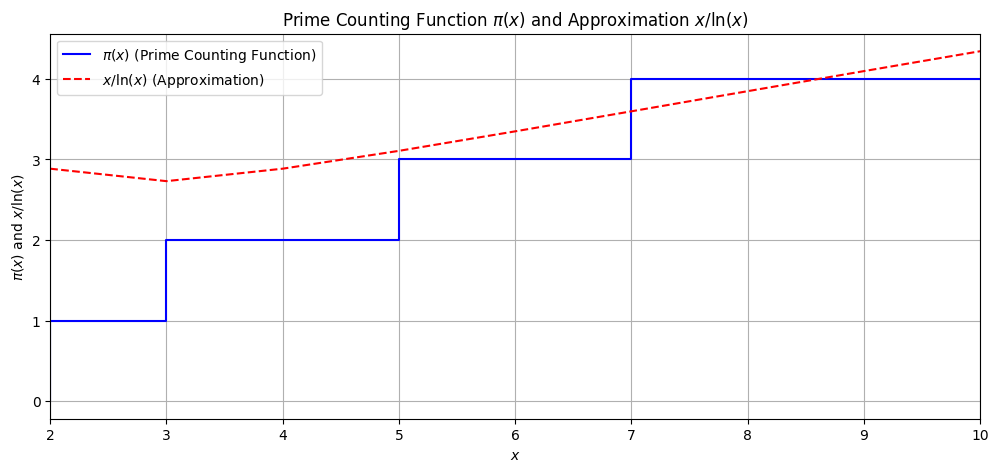
\includegraphics[width=.48\linewidth]{../Images/primecounting10}%
            \label{subfig:a}%
        }\hfill
        \subfloat[$x=500$]{%
            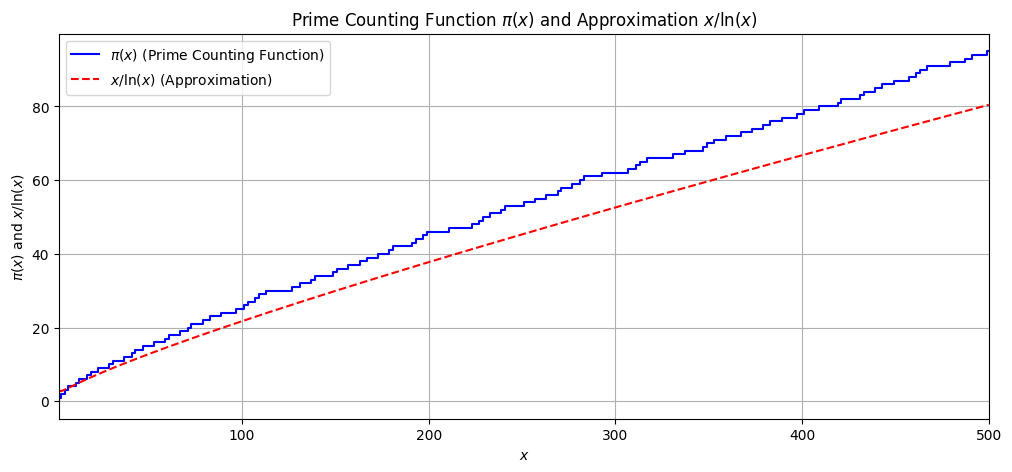
\includegraphics[width=.48\linewidth]{../Images/primecounting500}%
            \label{subfig:b}%
        }\\
        \subfloat[$x=1000$]{%
            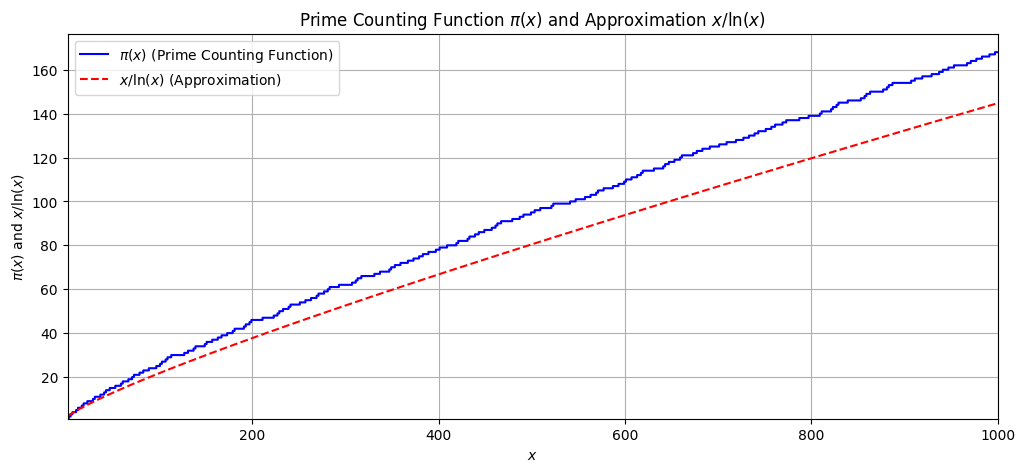
\includegraphics[width=.48\linewidth]{../Images/primecounting1000}%
            \label{subfig:c}%
        }\hfill
        \subfloat[$x=100000$]{%
            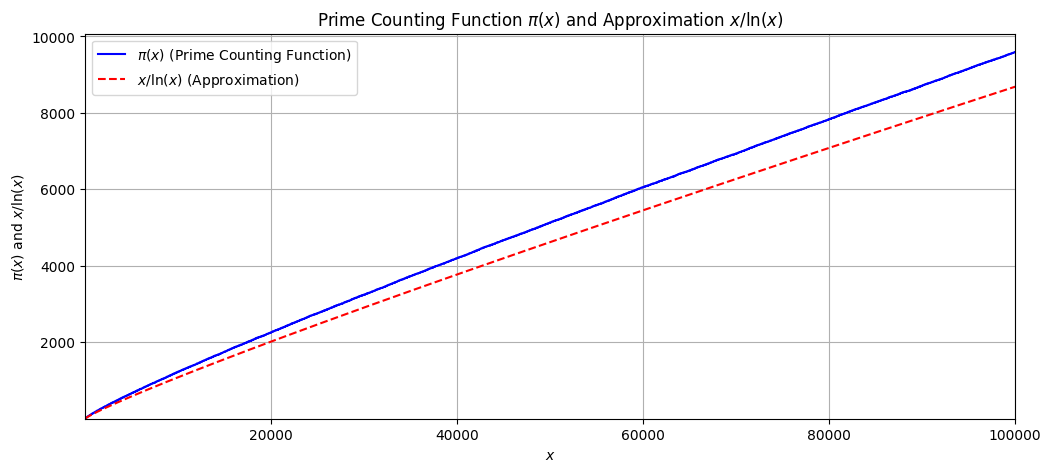
\includegraphics[width=.48\linewidth]{../Images/primecountingmax}%
            \label{subfig:d}%
        }
        \caption{Plots of different values of $\pi(x)$ and $\frac{x}{ln(x)}$}
        \label{fig:fig}
    \end{figure*}

\subsection{The prime number theorem}
$$\lim_{x\rightarrow\infty}\frac{\pi(x)}{\frac{x}{\ln(x)}} = 1$$
This means that as $x$ approaches infinity, the error between the 2 functions approaches to 0. However, The blue and red lines seem to be diverging, not converging as $x$ gets larger, does this mean the \textbf{the prime number theorem} is wrong? No, The theorem does not say that the difference $\pi(x) - \frac{x}{ln(x)}$ gets smaller as $x$ gets larger, instead what it does say is that the \textbf{ratio} between the approximation and the actual value gets closer to 1 as n gets larger and larger.
\begin{table}[h!]
\centering
\label{tab:prime_counting_ratio}
\[
\begin{array}{|c|c|c|c|}
\hline
x & \pi(x) & \frac{x}{\ln(x)} & \text{Ratio} \left(\frac{\pi(x)}{x/\ln(x)}\right) \\
\hline
10^2 & 25 & 22 & 88.00\% \\
10^3 & 168 & 145 & 86.31\% \\
10^4 & 1229 & 1086 & 88.36\% \\
10^5 & 9592 & 8686 & 90.55\% \\
10^6 & 78498 & 72382 & 92.21\% \\
10^7 & 664579 & 620421 & 93.36\% \\
10^8 & 5761455 & 5428681 & 94.22\% \\
10^9 & 50847534 & 48254942 & 94.90\% \\
10^{10} & 455052511 & 434294482 & 95.44\% \\
\hline
\end{array}
\]
\caption{Prime Counting Function, Approximation, and Ratio}

\end{table}


\begin{figure}[h!]
    \centering
    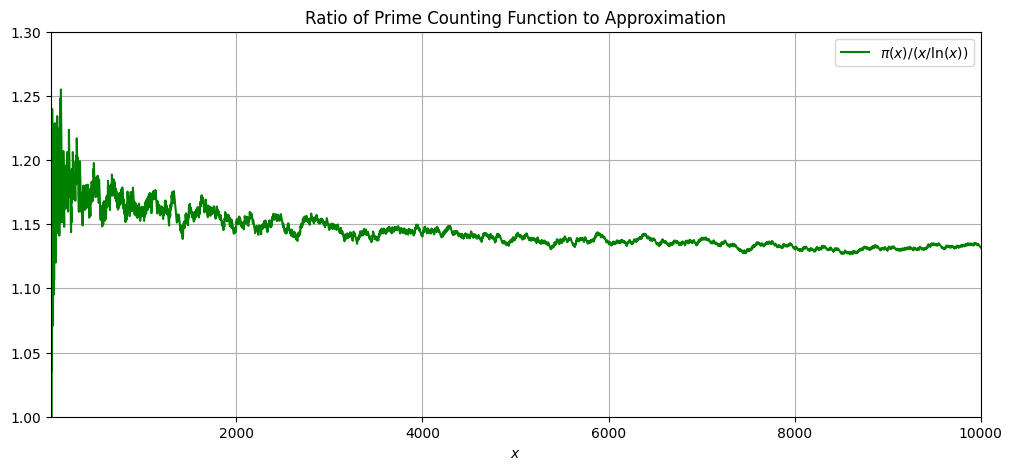
\includegraphics[width=0.8\linewidth]{../Images/ratio}
    \caption{graph of the ratio of the prime counting function and the approximation. }
    \label{fig:euler_zeta}
\end{figure}

\end{definition}
\newpage
%--------------------------------------------------------------------------------------------------------------

\section{prime numbers and computer science}

Prime numbers are natural numbers greater than 1 that is \textbf{not} a product of two smaller natural numbers (2, 3, 5, 7, 11...). In 300 BC Euclid demonstrated that there are infinitely many prime numbers. Prime numbers have puzzled mathematicians for thousands of years, several historical questions regarding prime numbers are still unsolved. Primes are used in several aspects of information technology such as public-key cryptography which replies on the difficulty of factoring large numbers into their prime factors.
\subsection{Cryptography} 	
\subsubsection{The RSA system}
The RSA algorithm is said to secure 90\% of the internet. The "s" is "https" means secure and the security is provided based on RSA. The RSA system in cryptography makes use of prime numbers to calculate its public and private keys. The strength of the system relies on the difficulty with the finding of the specific pair of prime numbers selected to create a large integer called the modulus. For example, 
if 11 and 17 are multiplied, it will give the number 187, when broken down, it will give the exact same 2 numbers. Therefore, the larger the number the stronger the encryption will be.
\subsection{Quantum Computing}
There is still no evidence that quantum computers can break numbers based on 1024 or 2048 encryption. Using the Riemann hypothesis would propose that prime numbers are divided predictably. Many mathematicians believe that the only accurate method of decryption is going to take place through quantum computing. There is a particular importance to prime factor factorization as the fundamental building block of all numbers. 
\subsection{Hash table}
Hashing is a standard algorithmic technique in computer algorithms that is used to reduce a large key into a small value that can be used as an index in a table. We use prime numbers so that the chances of two large keys matching the same index reduce. 
\\

The Riemann Hypothesis has many other important corollaries in Computer Science. In particular, the best known today deterministic test for the primality of a number p has complexity
$\Omega (p6)$ but already in 1976 G.L. Miller proposed an algorithm of complexity $O(p4)$ assuming the validity of the (extended) Riemann Hypothesis \cite{MATIYASEVICH2020257}.


%--------------------------------------------------------------------------------------------------------------

\section{Main Content}
In his 1859 paper, Bernhard Riemman wrote a short paper titled "On the Number of Primes Less Than A Given Magnitude". Where he introduced the connection between the prime counting function $\pi(x) $ and the Riemann Zeta function $\zeta(s)$. He discovered a hidden relation between the distribution of primes and the zeros of his zeta function.
 

%-------------------------------------------------------------------------------------------------------------

\subsection{Analytic continuation}
Riemann used a advanced technique called analytic continuation to extend the domain of a function, He used this to extend the domain of Euler's zeta function.

\begin{figure}[h!]
    \centering
    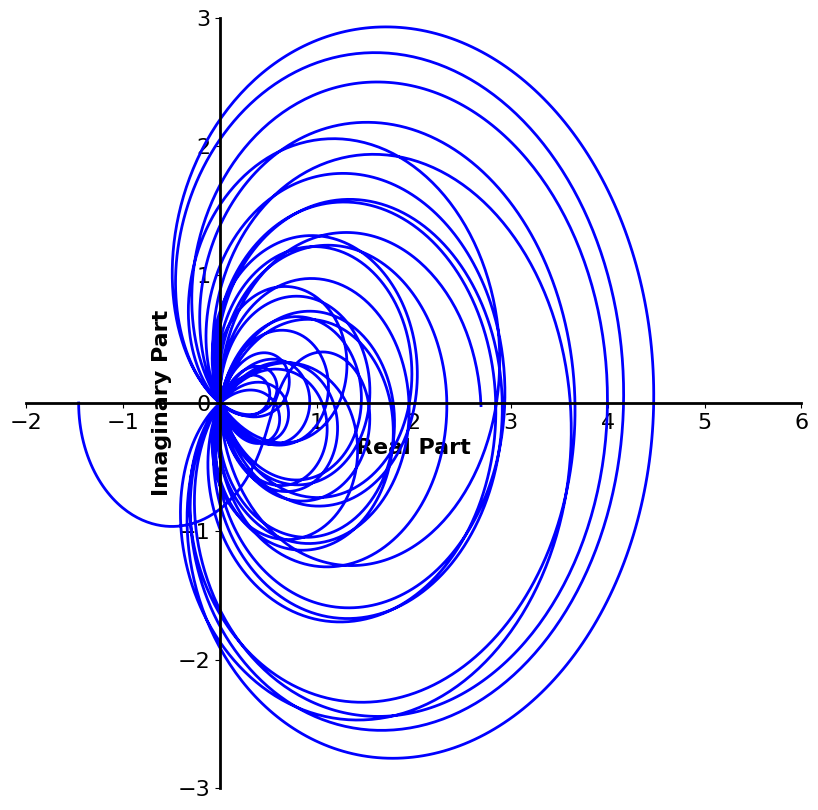
\includegraphics[width=0.8\linewidth]{../Images/zetafunction}
    \caption{Zeta Function}
    \label{fig:euler_zeta}
\end{figure}
When Riemann extended the domain, in the new territory, the $\zeta(s)$ function can be seen crossing through the origin, what this means is that for some values, the $\zeta(s)$ function evaluates to 0, we call these \textbf{zeta zeros}. Some zeros are easy to find, when you input an even negative integer, you will get a zero. We call these the "trivial zeros". We do not care about these trivial zeros, what we are interested in are the non trivial zeros.
\subsection{Riemman zeta function }
The complex 

\subsection{The Riemann Hypothesis}  These other zeta zeros exhibit a very compelling pattern, all the non trivial zeros lie within a single region called the \textbf{critical strip}, where $0\le s \le 1 $. Riemann proved that there are infinitely many zeros in the critical strip. Riemann hypothesized that all the non trivial zeros are not just anywhere in the strip but on a single vertical line, called the \textbf{critical line} which is where the $\Re(s) = \frac{1}{2}$. More formally,

\\

\noindent\fbox{%
    \parbox{\textwidth}{%
        \textbf{The Riemann hypothesis} states that the zeros of the zeta function that lie between $0 \leq s \leq 1$ have $\operatorname{\Re}(s) = \frac{1}{2}$.
    }%

}
\\

This is the million dollar problem. This statement is actually the crux of understanding the distribution of prime numbers.  At this point, you might be asking yourself "what does this have to do with prime numbers?"

\section{Riemann's Hypothesis shows the distribution of prime numbers can be predicted}
Let us continue with the assumption that the Riemann hypothesis holds, that is all non-trivial zeros of $\zeta(s)$ have real part equal to 1/2. We can now separate the sum over all zeros into a sum over non-trivial zeros and a sum over trivial zeros. We will end up with 
$$\psi_0(x) + \log(2\pi) = x- 4\sqrt{x}\sum_\gamma{\frac{\cos(\gamma \log(x))+2\gamma \sin(\gamma \log(x)))}{1+4\gamma^2}} -\frac{1}{2}\log(1-x^{-2})$$
Now let us plot this equation, this will allow us to clearly see the effect of including increasingly more zeros of the zeta function. Using the formula, one can approximate the number of primes up to and including a given number x to a very high accuracy. In fact, Von Koch proved that using the non-trivial zeros of the Riemann zeta function to error-correct the function is the "best possible" bound for the error term in the prime number theorem.
    
   \begin{figure*}[h!]
        \subfloat[$0$ non trivial zeros]{%
            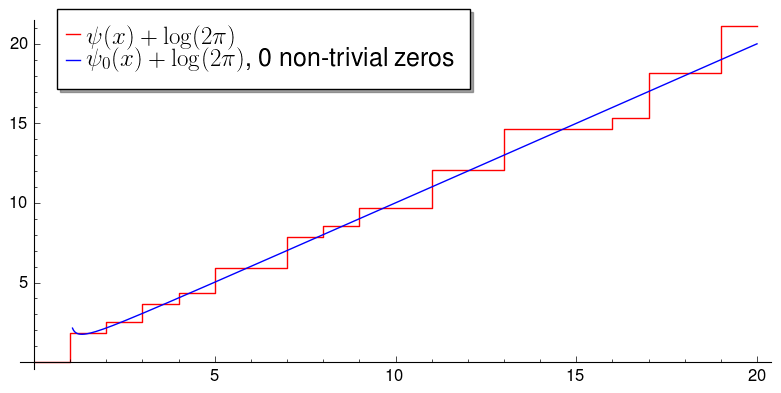
\includegraphics[width=.48\linewidth]{../Images/0ntz}%
            \label{subfig:a}%
        }\hfill
        \subfloat[$1$ non trivial zeros]{%
            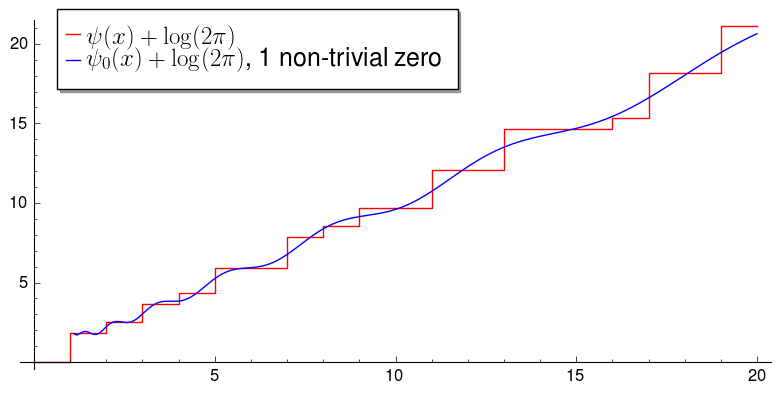
\includegraphics[width=.48\linewidth]{../Images/1ntz}%
            \label{subfig:b}%
        }\\
        
        \subfloat[$10$ non trivial zeros]{%
            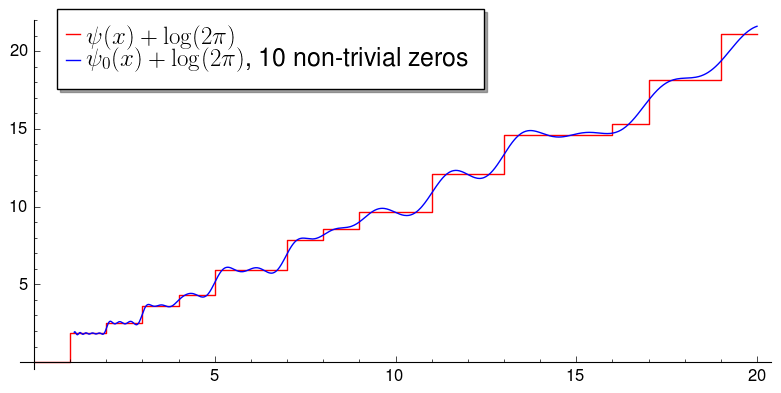
\includegraphics[width=.48\linewidth]{../Images/10ntz}%
            \label{subfig:c}%
        }\hfill
        \subfloat[$100$ non trivial zeros]{%
            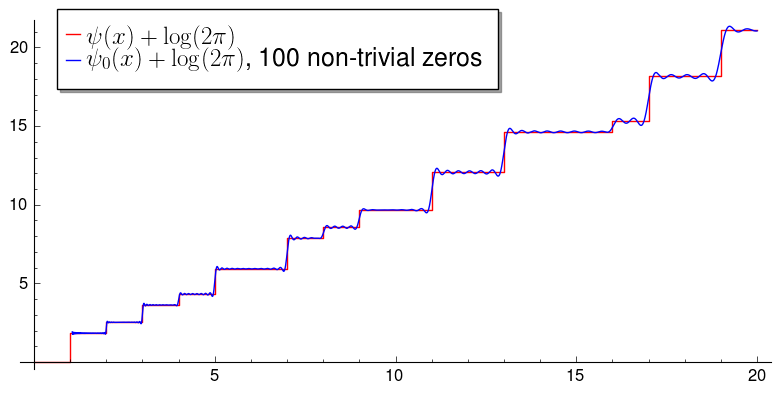
\includegraphics[width=.48\linewidth]{../Images/100ntz}%
            \label{subfig:d}%
        }
        \caption{Plots of prime counting function with non trivial zeros as a error term.}
        \label{fig:fig}
    \end{figure*}
    
   
   
   This clearly shows that the more non trivial zeros we add, the better the approximation for the prime counting function is. This is why the Riemann hypothesis is so important, if the hypothesis is true, the distribution of prime numbers is as regular as possible and can be predicted. Deviations in the zeros from the critical line would imply irregularities in the spacing of primes. Researches have computed trillions of non trivial zeros in the zeta function and all of them thus far have been found on the critical line $\Re(\frac{1}{2})$. 
%--------------------------------------------------------------------------------------------------------------

%--------------------------------------------------------------------------------------------------------------
\section{Conclusion}

%--------------------------------------------------------------------------------------------------------------

%--------------------------------------------------------------------------------------------------------------
% REFERENCES
%--------------------------------------------------------------------------------------------------------------
\bibliographystyle{plain}
\bibliography{bibliography}

\end{document}
